% This is the Reed College LaTeX thesis template. Most of the work
% template. Later comments etc. by Ben Salzberg (BTS). Additional
% restructuring and APA support by Jess Youngberg (JY).
% Your comments and suggestions are more than welcome; please email
% them to cus@reed.edu
%
% See http://web.reed.edu/cis/help/latex.html for help. There are a
% great bunch of help pages there, with notes on
% getting started, bibtex, etc. Go there and read it if you're not
% already familiar with LaTeX.
%
% Any line that starts with a percent symbol is a comment.
% They won't show up in the document, and are useful for notes
% to yourself and explaining commands.
% Commenting also removes a line from the document;
% very handy for troubleshooting problems. -BTS

% As far as I know, this follows the requirements laid out in
% the 2002-2003 Senior Handbook. Ask a librarian to check the
% document before binding. -SN

%%
%% Preamble
%%
% \documentclass{<something>} must begin each LaTeX document
\documentclass[12pt,twoside]{reedthesis}
% Packages are extensions to the basic LaTeX functions. Whatever you
% want to typeset, there is probably a package out there for it.
% Chemistry (chemtex), screenplays, you name it.
% Check out CTAN to see: http://www.ctan.org/
%%
\usepackage{graphicx,latexsym}
\usepackage{amsmath}
\usepackage{amssymb,amsthm}
\usepackage{longtable,booktabs,setspace}
\usepackage{chemarr} %% Useful for one reaction arrow, useless if you're not a chem major
\usepackage{rotating}

% Modified by CII
\usepackage[hyphens]{url}
\usepackage{hyperref}
\usepackage{lmodern}

% Added by CII (Thanks, Hadley!)
% Use ref for internal links
\renewcommand{\hyperref}[2][???]{\autoref{#1}}
\def\chapterautorefname{Chapter}
\def\sectionautorefname{Section}
\def\subsectionautorefname{Subsection}

\usepackage{caption}
\captionsetup{width=5in}

% \usepackage{times} % other fonts are available like times, bookman, charter, palatino

\title{Consumption and Cooptation of Care: a statistical analysis of visits to
urgent care}
\author{Kaitlyn R. Jackson}
% The month and year that you submit your FINAL draft TO THE LIBRARY (May or December)
\date{May 2016}
\division{History and Social Sciences}
\advisor{Jessica F. Epstein}
%If you have two advisors for some reason, you can use the following
%\altadvisor{Your Other Advisor}
%%% Remember to use the correct department!
\department{Sociology}
% if you're writing a thesis in an interdisciplinary major,
% uncomment the line below and change the text as appropriate.
% check the Senior Handbook if unsure.
%\thedivisionof{The Established Interdisciplinary Committee for}
% if you want the approval page to say "Approved for the Committee",
% uncomment the next line
%\approvedforthe{Committee}

% Below added by CII

%%% Copied from knitr
%% maxwidth is the original width if it's less than linewidth
%% otherwise use linewidth (to make sure the graphics do not exceed the margin)
\makeatletter
\def\maxwidth{ %
  \ifdim\Gin@nat@width>\linewidth
    \linewidth
  \else
    \Gin@nat@width
  \fi
}
\makeatother

\renewcommand{\contentsname}{Table of Contents}

\setlength{\parskip}{0pt}

\providecommand{\tightlist}{%
  \setlength{\itemsep}{0pt}\setlength{\parskip}{0pt}}

\Acknowledgements{
I want to thank a few people, mostly my mom for going days without me
remebering to answer my phone and then always being there when I needed
an ear to whine to. I love you I love you I love you.
}

\Dedication{
To Reed: as an institution, as a moment in time, as a community, and as
a home. This is probably as cheesey as it gets, but damn this place is
special. My experiences here has changed me in some fundamental,
unmoveable way and I'll never forget it.
}

\Preface{

}

\Abstract{
Urgent care centers are a relatively new and emergent phenomemnon in the
American health care system, yet little to no academic reasearch has
been performed on how they are situated in the larger sociological
understanding of the healthcare system. This thesis attempts to further
such an understanding by examining the typologies of patients which are
the users of urgent care, and further, who of those uses such centers as
their primary care physicians.
}

\usepackage{tikz} \usepackage{setspace} \pagestyle{plain}

%%
%% End Preamble
%%
%

\begin{document}

      \maketitle
  
  \frontmatter % this stuff will be roman-numbered
  \pagestyle{empty} % this removes page numbers from the frontmatter

      \begin{acknowledgements}
      I want to thank a few people, mostly my mom for going days without me
      remebering to answer my phone and then always being there when I needed
      an ear to whine to. I love you I love you I love you.
    \end{acknowledgements}
  
  
  % Add table of abbreviations?

      \hypersetup{linkcolor=black}
    \setcounter{tocdepth}{2}
    \tableofcontents
  
  
  
      \begin{abstract}
      Urgent care centers are a relatively new and emergent phenomemnon in the
      American health care system, yet little to no academic reasearch has
      been performed on how they are situated in the larger sociological
      understanding of the healthcare system. This thesis attempts to further
      such an understanding by examining the typologies of patients which are
      the users of urgent care, and further, who of those uses such centers as
      their primary care physicians.
    \end{abstract}
  
      \begin{dedication}
      To Reed: as an institution, as a moment in time, as a community, and as
      a home. This is probably as cheesey as it gets, but damn this place is
      special. My experiences here has changed me in some fundamental,
      unmoveable way and I'll never forget it.
    \end{dedication}
  
  \mainmatter % here the regular arabic numbering starts
  \pagestyle{fancyplain} % turns page numbering back on

  \chapter*{Introduction}\label{introduction}
  \addcontentsline{toc}{chapter}{Introduction}
  
  \onehalfspacing
  
  The past two decades have seen a surge in a new form of medical
  practice: walk in clinics designed with an emphasis on acute, quick and
  cheap care.
  
  This thesis asks the question, what are the typologies of patients using
  these centers, what and how can we use this information to situate
  urgent care centers into the larger complex of the American helathcare
  system? These questions are particuarly pressing, because as the rapid
  exapansion of the industries continues, there has been little
  sociological reasreach on their effect
  
  There is no official definition of what constitutes an urgent care
  center, but the scope of services provided generally falls between that
  of a primary care doctor's office and an emergency department. These
  urgent care centers focus on acute episodic care with a substantial
  emphasis on customer service.
  
  The first of these centers opened in the United States in the early
  1980's., with no more than a handful in operation at the time.
  Unfortunately, (at least as far as early investors were concerned), the
  industry rapidly declined, and the few clinics which had opened were
  largely obsorbed into larger hospitals and healthcare groups. Ten years
  later, in the mid-1990's , the industry again began growing rapidly,
  growing to between 12,000 and 20,000 centers today. By the UCAOA's
  estimate, in 2014 approximately two new urgent care centers were opening
  in the United States each week.
  
  Such recent and rapid expansion of the industry has been heavily
  examined by the media, which often attribute growth to a diverse set of
  market factors such as long wait times for primary care appointments,
  crowded emergency departments and patient demand for more accessible
  care, including after-hours appointments (Yee, Lechner, and Boukus
  2013). Yet despite the rapid development of the industry and the great
  interest sociologists have historically taken in America's health care
  system, hardly any scholarly research has been done on why these centers
  are coming to play a major part of the healthcare system or what their
  patterns of use are. While many are quick to point towards long wait
  times, and the difficulty of finding doctors in the current healthcare
  system, the repurcussions of the new turn torwards urgent care centers
  are not well known, nor has their place in the American healthcare
  system been examined.
  
  In the following analysis, I will attempt to situate the rise of such
  clinics within the existing sociological research on the American
  healthcare system, examining hypotheses about how the patterns of use by
  patients at these centers can help us understand and situate them in to
  the larger American healthcare complex. To do this, I compare three
  understandings of urgent care centers
  
  In Chapter one, I highlight the rise in the number of urgent care
  centers in the United States since the early 1990's, showing the rising
  prominence of these institutions. I also provide background on the
  services and care these faciilities offer, focusing on how they are
  advertised and their own obvious institutional goals. I situate urgent
  care centers into a wider context of the American healthcare system's
  varied actors and organizations, and explore the ways these insitutions
  might offer a response to common complaints regarding the accessibility
  and organization of the more established healthcare faciliites.
  
  Chapter two turns to the current sociological understandings of the
  healthcare system, and examines how the competing theories of the
  patient/doctor relationship work when examining these actors in an
  urgent care setting, focusing on theories of consumerism in modern
  healthcare. I highlight how these new organizations might informally
  facilitate an arm's length relationship between practitioner and
  patient, eliminating the close ties many medical sociologists have
  identified as vital to an optimal doctor patient relationship. In this
  chapter I also highlight the current gaps in the literature surrounding
  new forms of medical care facilities which have been largely ignored by
  sociologist and other scholars attempts to understand health care in
  America.
  
  Chapter three offers a description of the National Ambulatory Medical
  Care Survey where I am drawing my anlysis from, and including a
  description of the methods I use to examine patient visits to urgent
  care. These include both a k-modal hieracrchal clustering exploratory
  analysis used to identify groups of similar patients using urgent care
  and a logistic analysis of those choosing to use urgent care as their
  primary care facility. Chapters four and five present these analyses,
  and discuss the findings in light of the research.
  
  In the conclusion, I explore the implications of the tensions between
  what is thought important to the doctor-patient relationship, and the
  reality of accessing healthcare in America today. I argue that\ldots{}
  ** really need to clarify what I'm arguing here **. I conclude with
  implications and suggestions for ways in which urgent care centers could
  be incorporated into the traditional healthcare model.
  
  \chapter*{Theoretical and Historical
  Foundations}\label{theoretical-and-historical-foundations}
  \addcontentsline{toc}{chapter}{Theoretical and Historical Foundations}
  
  \onehalfspacing
  
  In this chapter, the quantitative, visit level analysis of urgent care
  centers that follows later will be situated in the longer-term primarcy
  care trends of the American healthcare system. The existing sociological
  research on the patient and practioner, and how this has changed over
  the last half-century, are vitally impotant to beggining to understand
  how urgent care centers may be operating, as changes in the last half
  century have had drastic effect on this relationship. To understand the
  how and the why of urgent care centers, one must have some inkling of
  the complicated and tangled history of the medical profession in the US,
  and how infrastructural changes and epistomological shifts have led to
  the current state of affairs. To begin with, the chapter returns to the
  traditional tales of the primary care physician \emph{still} visible in
  modern sociological texts on healthcare. Tracing the development and
  subsequent decline of medical professional power, I then review much of
  the current literature regarding the consequences of such structural
  changes on the doctor/patient relationship. These changes lead us to the
  current epistomology of American healthcare, and I review theories on
  the patient as consumer which strengthen the argument that urgent care
  centers can and \emph{should} be studied by academics interested in the
  field.
  
  \subsection*{The man, the myth, the legend:
  \textbackslash{}Understanding the Doctors of
  Yesteryear}\label{the-man-the-myth-the-legend-understanding-the-doctors-of-yesteryear}
  \addcontentsline{toc}{subsection}{The man, the myth, the legend:
  \textbackslash{}Understanding the Doctors of Yesteryear}
  
  In 2006, the Millis report (Unknown), commisioned by the American
  Medical Association, was asked to review the current status of
  physicians in the US. In the first section, the recalled the physician
  of revered memory in America:
  
  \singlespace
  
  \begin{quote}
  ``The general practitioner of revered memory knew his patients\ldots{}
  and provided continuing care through the course of minor ailments and
  majors emergencies. His deficiencies\ldots{} were partly offset by
  intimate knowledge of his patients, the support he gave them, and the
  trust and confidence his services engendered.''
  \end{quote}
  
  \onehalfspacing
  
  Such a view of the doctor occurs profusely throughout early to mid
  twentieth century literature on the profession, and is even visible
  today, though often as a thing to be reminisced, or a goal to return to.
  A person's doctor, traditionally, was an extrememly integrated, close,
  and important connection in a person's life. This was a relationsihp
  built, for some on trust, agency, and mutual understanding, while for
  others on power imbalance, technocratic authority and affective
  neutrality.
  
  Importantly, in both cases the doctor is an embedded social tie in the
  patient's life.
  
  \emph{Insert name}
  
  \section*{The end of Medical Professional Dominance in the
  US?}\label{the-end-of-medical-professional-dominance-in-the-us}
  \addcontentsline{toc}{section}{The end of Medical Professional Dominance
  in the US?}
  
  Almost since sociologists first became interested in the medical
  profession, the sociology of medicine was deeply joined with studies of
  professionalism. In the U.S., Doctors were seen as the paragon of the
  `professional': respected, organized, in control, and above all else,
  firmly established in their positions. Such traits led many to study
  what effects this had on medical care and how such professional
  dominance of medical practitioners shaped what services were provided.
  Many found that such dominance allowed the profession to block off areas
  of study entirely, or to ignore diseases they did not want to pursue.
  Such ``modern doctors'' worked within a ``sovereign profession'' (Starr
  1982), serenely dispensing both medical care and authoritative judgment.
  Freidson (1988, p.384) comments that before 1970's, U.S. medicine ``was
  at a historically unprecedented peak of prestige, prosperity and
  political and cultural influence---perhaps as autonomous as it is
  possible for a profession to be.''
  
  When one thinks of the healthcare industry today, it is hard to call to
  mind such professional cohesion. While doctors remain one of the more
  highly respected career choices in America, their prestige has certainly
  dropped since the 20th century (Heritage and Maynard 2006). The term
  doctor is now applicable to a wide variety of sub-professions and
  specialties and the medical profession has become extremely diversified.
  Along with such specialization, big changes to Medicare and Medicaid
  legislation and the growth of third-party payers and for-profit medical
  service corporations created conditions which further removed the doctor
  from their traditional roles, eroding the political and cultural
  influence of the profession and threatening the cultural authority and
  technical autonomy of medicine (Starr 1982, Freidson 1988). It should be
  noted that such changes may not have necessitated a loss of professional
  dominance. In fact, with the expansive growth on spending in the
  healthcare sector, it is possible that doctors could have further
  cemented their professional medical authority. But most scholars have
  observed that the opposite has happened, and instead many view the past
  30 years as the end of the authoritative medical professional.
  
  With such a history of professional prominence, many have examined the
  observed decline in depth, and the change is largely seen as a
  consequence of a loss of trust with the medical profession as a whole
  that began some time around the late 1970's (Timmermans and Oh 2010).
  During the `golden age', public surveys reported extremely high levels
  of trust in physicians, however this declined from 72 percent in 1966 to
  37 percent in 1981 (Lipset and Schneider 1982). With high levels of
  doubt towards medical professionals, suspicion grew about physicians
  acting in patients' best interests (Reeder 1972) and patients began to
  question the validity of the medical doctor as an authoritative figure
  of biological truth.
  
  These shifts in the medical profession occurred parallel to changing
  norms surrounding the role of the patient in their own health care, and
  the last 30 years of scholarly research have seen a reconfiguration of
  the patient from passive recipient of care from their doctor to a
  critical consumer of health services (Barker 2008; Lupton, Donaldson,
  and Lloyd 1991; Timmermans and Oh 2010). Theories of medical consumerism
  developed from economists studying the healthcare sector, and they begin
  with a similar hypothesis as the economic rational choice model,
  assuming that patients act as rational actors in the context of a
  medical encounter (Timmermans and Oh 2010). In other words, individuals
  act in a calculated manner to engage in self-improvement or health, and
  they are generally skeptical about expert knowledge (Lupton 1997).
  According to the literature, this trend began to express itself in the
  form of solicitation of second opinions and a sense of
  interchangeability of medical practitioners during the 1980's, just as
  distrust of the industry reached its peak (Gray 1997). The idea that
  patients could shop around and compare services and prices was heavily
  popularized, and patients increasingly began to make autonomous
  decisions when selecting physicians (Hibbard and Weeks 1987, Lupton
  1991).
  
  Urgent care centers fit neatly into such a conceptualization of health
  services, and thus offer a key area of analysis in better understanding
  the developing roles of the consumer-patient within the larger
  healthcare industry. An important aspect of the research on the
  developing patient-consumers emphasizes the expansion of bargaining
  power on the part of the patient that came with the shift (Reeder 1972).
  A patient may now shop around the marketplace of health care, and that
  many are now choosing urgent care centers is undeniable given the
  industry's rapid expansion.
  
  \section{Primacy of Primary Care}\label{primacy-of-primary-care}
  
  Turning away from the fate of doctoring, it is important to ackknoledge
  that the fate of primary care physicians has been reported to be hanging
  in the balance for quite some time. In 2006, the American College of
  Physicians released a report with the ominous title ``The Impending
  Collapse of Primary Care Medicine and Its Implications for the State of
  the Nation's Health Care'' (ACP, 2006)
  
  \section*{Moving away from Primary
  Care}\label{moving-away-from-primary-care}
  \addcontentsline{toc}{section}{Moving away from Primary Care}
  
  The shift towards urgent care centers will undoubtedly have profound
  consequences for the patient-practitioner relationship and the patient's
  role in the medical care system, but so far these consequences remain
  largely unknown. Fortunately, sociologists have had a long-standing
  concern with such professional-client interactions, particularly within
  medicine (Freidson 1961, Bloom 1963, Mechanic 1968), and in order to
  better understand what effects the shift away from primary care may have
  on patients, one can look to a large body of research on how
  institutional and organizational environments directly affect a
  patient's experience in health care.
  
  A major sociological theory of the doctor-patient relationship begins by
  speculating that the bureaucratization of modern social institutions has
  had drastic consequences on the medical profession: as opportunities for
  close personal contacts diminish, problems which were originally handled
  in familial, social, and religious contexts are transferred to `formal
  sustaining practitioners' (Mechanic 1966). In such societies, the
  prescribed structure of the doctor patient relationship then provides a
  legitimation for the expression of intimacy and the request for help,
  offering an explanation as to why sociologists and anthropologists of
  medicine have long observed the variance and social nature of health
  problems brought to a physician (The Doctor, His Patient, and the
  Illness).
  
  These same theorists locate the stability of this doctor-patient
  relationship in the fact that the physician acts as the patient's agent,
  yet one can immediately recognize that urgent care centers may not be
  equipped to facilitate this relationship in the same way that the
  traditional primary care practice is seen to (Lupton 1997). The premise
  of urgency in such practices, the quickness with which patients are
  seen, and the targeted focus on acute problems all serve to create
  considerable doubt towards the ability of physicians within such an
  organizational context to fulfill the sociological role thought so
  important in previous literature.
  
  Additionally, those who study health services have recognized that a
  patient's medical history is a primary source of information regarding
  treatment, and primary care practitioners have been known to draw upon
  this as a valuable resource (Draper and Smits 1975; Miller et al. 2010).
  
  Urgent care centers however have no emphasis on maintaining
  patient-doctor ties and there is no reliable system to ensure a patient
  sees the same doctor even if they have been there before.
  
  Yet while this may seem problematic, a large body of recent sociological
  literature belongs to a growing number of scholars who are challenging
  the importance, and even relevance, of the traditional primary care
  physician in modern medicine. Those who have been observing developments
  in the patient-physician relationship over the past 30 years argue that
  the last quarter of the 20th century saw a dramatic reconfiguration of
  society, especially in regards to health services, which has had
  profound effects on an individual's relationship to the healthcare
  system. So while some were witnessing what was, for Starr (1982), ``the
  social transformation of medicine,'' and for many, ``the end of the
  golden age of doctoring'' (McKinlay \& Marceau 2002).
  
  \subsection*{What does this mean for health
  care?}\label{what-does-this-mean-for-health-care}
  \addcontentsline{toc}{subsection}{What does this mean for health care?}
  
  In light of such research, sociologists and those who study at the
  intersection of health and social behaviors have begun to re-examine the
  importance of a close relationship between doctor and patient in an
  attempt to respond to the consumer-patient model, developing a growing
  body of research which seeks to define the most effective components of
  patient-physician interactions and to reaffirm the place of the primary
  care physician in modern medicine. Common to most of these studies are
  the elements of `trust, compassion, communication, and clinical
  competence' (Heritage and Maynard 2006; Phillips and Bazemore 2010,
  others at bottom). As an example, a 2002 study on clinical outcomes for
  low income women over the age of forty found that women who rated
  highest their doctor's ability to take care of all of their health care
  needs had 11 times the odds of `trusting their physician' and 6 times
  the odds of finding their physicians `compassionate and communicative',
  compared to those with the lowest level of comprehensiveness (O'Malley
  and Forrest 2002).
  
  With such knowledge that close ties between physicians and patients have
  a direct impact on the perceived quality of care, the importance of
  examining the rise of urgent care centers become obvious. If patients
  are acting as rational consumers, which of them are choosing to receive
  their care outside of a primary care office, and what consequences does
  this have for their medical outcomes? The lack of research into the
  characteristics of urgent care patients make it difficult to answer such
  questions. Indeed, as of now, there has been no academic attempt to
  place the rapidly growing industry within the sociology of medicine, nor
  does there even exist an official definition of what constitutes an
  urgent care center.
  
  \chapter*{Theories of Urgent Care
  Use}\label{theories-of-urgent-care-use}
  \addcontentsline{toc}{chapter}{Theories of Urgent Care Use}
  
  \onehalfspacing
  
  Urgent care centers are an obviously understudied phenomenon, and the
  following section applies sociological theories to better understand
  their role in the healthcare system.
  
  \subsection*{Urgent Care Centers as an extension of the Welfare
  State}\label{urgent-care-centers-as-an-extension-of-the-welfare-state}
  \addcontentsline{toc}{subsection}{Urgent Care Centers as an extension of
  the Welfare State}
  
  The prevailing understanding of urgent care centers interprets the
  industry's growth as a development that grew out of emergency department
  overcrowding that began during the financial tightening of the 1980's.
  Thus, each clinic is often conceptualized as a smaller instance of a
  traditional hospital's triage center, supplying many services which one
  could receive at an emergency department (Anon n.d.; Mehrotra et al.
  2008; Rubin 2012). One study which compared emergency department
  services with urgent care centers found that, for all but the most
  extreme care and emergent care needs, urgent care centers could handle
  almost all of emergency department traffic and that their services were
  remarkably analogous (Anon n.d.). Similarly, the unique features of
  emergency departments which set them apart from more traditional avenues
  of care such as the promise to be seen regardless of insurance coverage
  and the flexible hours are mirrored in most urgent care centers (Weinick
  and Betancourt n.d.).
  
  Given these similarities, urgent care could in many ways be considered a
  response by the healthcare industry to emergency department overuse,
  which continue to struggle underneath a lack of resources. Suitably, the
  body of sociological research on emergency departments can be used to
  better comprehend how urgent care centers are impacting the allocation
  of healthcare. Many medical sociologists have analyzed the
  public/private divide in the healthcare industry, emphasizing the
  unequal quality of care received depending upon which type of health
  service you utilize (Dutton 1978; Luftey and Freese 2005). In response
  to these inequalities in the private sector, the emergency room has long
  been understood as a response to a stratified system, and it is largely
  considered a social welfare institution (Gordon 1999). ``The hospital
  emergency department is perhaps the only local institution where
  professional help is mandated by law, with guaranteed availability for
  all persons, all the time, regardless of the problem'' (Ullman, Block,
  and Stratmann n.d.), and was for a long time widely considered one of
  the few access points into the healthcare system for very low income
  individuals.
  
  Accordingly, because urgent care centers offer a similar alternative to
  primary care for those who cannot procure a conventional family
  practitioner, they can be considered an extension of a much needed
  welfare institution necessary to circumvent an extremely stratified
  healthcare industry. This becomes more credible when trends in urgent
  care centers are examined in conjunction with emergency departments. By
  all indications, the demand for emergency departments far outweighs
  their capacity, and this is only expected to grow in the future (Weinick
  2010). Around the time that urgent care centers began to emerge in the
  U.S., emergency departments were seeing record breaking levels of
  non-acute visits, resulting in severe overcrowding and shortages
  (Shortcliffe). These numbers have only risen in the past 20 years,
  especially in urban areas with large populations of low-income residents
  (Anon n.d.). Not only does this rise in demand correspond to the growth
  of the urgent care industry, one economic analysis which took cities
  with comparably high levels of non-emergent ED usage and examined the
  effect of a growing number of urgent care centers found that cities
  which have seen a large growth in these facilities have statistically
  lower overcrowding in emergency departments (O'Malley 2013).
  
  Thus, urgent care centers usage would be expected to closely resemble
  that of the emergency department, especially regarding non-emergent
  care. This leads to the first hypothesis which will be tested by current
  data on urgent care center usage. Emergency department usage has been
  studied by many medical professions and sociologists, with a particular
  focus on the ways in which it serves as a welfare institution, and a few
  central patterns will be used here in the comparison with urgent care
  centers. Primarily, the low average income of patients and high levels
  of uninsured visits to emergency department patients have been a steady
  trend in the last 30 years (Ullman et al. n.d.). Patterns of use for
  emergency departments also show low levels of `returns' (individuals who
  come back with the same problem) and higher traffic during hours when
  normal primary care physician offices are closed, such as late at night
  and on the weekend (Anon n.d.; O'Malley 2013; Ullman et al. n.d.).
  Accordingly, if like emergency departments, urgent care centers act as a
  a welfare institution for those who cannot procure a traditional primary
  care physician, we would expect to see similar trends as have been
  observed in hospital emergency departments. These are summarized in
  Hypothesis 1 below.
  
  \paragraph{Hypothesis 1: Urgent care centers will experience high levels
  of visits from uninsured and low SES patients, have low rates of second
  visits, and higher rates of visits during non-traditional hours
  (weekends).}\label{hypothesis-1-urgent-care-centers-will-experience-high-levels-of-visits-from-uninsured-and-low-ses-patients-have-low-rates-of-second-visits-and-higher-rates-of-visits-during-non-traditional-hours-weekends.}
  
  \subsection*{Urgent Care Centers as a New Model of Primary
  Care}\label{urgent-care-centers-as-a-new-model-of-primary-care}
  \addcontentsline{toc}{subsection}{Urgent Care Centers as a New Model of
  Primary Care}
  
  Yet another understanding of urgent care centers arises when one
  considers the larger institutional context within which the overuse of
  emergency departments and the boom in the urgent care industry occurred.
  According to medical and organizational sociologists, the institutional
  narrative of the American healthcare industry since the 1980's is one of
  privatization and the transfer of power from professionals and the
  government towards the private sector and market control (Waitzkin
  2000). Urgent Care centers thus fall into a rapidly expanding category
  of new, privately funded modes of healthcare services---other examples
  being retail clinics, private hospitals and home care
  organizations---which are provided and predominantly paid for by private
  actors (Anon n.d.).
  
  This framework has yet to be fully examined by scholars, but a few
  studies which have attempted to examine the place of urgent care centers
  in new healthcare markets have pointed towards such change as being
  highly indicative of larger changes to healthcare, highlighting the
  privatization phenomenon as a possible explanation in the rise in
  numbers of such clinics over the last two decades or so (Rubin 2012;
  Weinick, Bristol, and DesRoches 2009; Yee et al. 2013). Shortages in
  public hospital staffing and facilities and the rising cost of care in
  the U.S. are seen as having created both demand and an opening for a new
  market within healthcare, which has been filled by new forms of medical
  service (Weinick and Betancourt n.d.). And while the trend towards
  privatization has been seen at times as both a symptom of the loss of
  professional dominance by medical practitioners and the cause of it, the
  similarities in organizational structure to primary care practices cast
  doubt on the hypothesis that these new forms of care are simply
  emergency department overflow. As one analysis observed: ``while urgent
  care reflects some similarities to emergency departments, we find that
  in other areas -- most notably reimbursements, primary payer
  distribution, and physicians' salaries -- urgent care centers seem far
  more similar to office-based family medicine practices'' (Weinick and
  Bristol 2008).
  
  Such observations lead one to a different conclusion about urgent care
  than those who liken the clinics to smaller triage centers created to
  handle emergency department overflow. Instead, urgent care centers can
  be conceptualized as a move by the healthcare industry towards deeper
  privatization, and possibly a response to medical professional authority
  in jeopardy. When medical sociologists first began pointing to ``the end
  of the golden era of doctoring,'' Stefan Timmermans responded by
  pointing to the long history of adaptability by the medical profession,
  which has managed to transform itself before in the wake of
  institutional change many times before (Timmermans, Whooley).
  
  Consequently, if the privatization of healthcare proves to be the
  primary explanation of why urgent care centers are beginning to dominate
  the acute-care market, one would expect to see trends in use mirror
  those of traditional primary care physicians rather than emergency
  departments. Historically, primary care often acted as a first contact
  point for insured patients for any acute, non-emergent health concerns
  of these individuals (Jost 2003). While many primary care offices will
  accept at least a small number of Medicaid and Medicare payments, they
  often have a large patient base of privately insured, financially
  well-off individuals (Cunningham et al. 1999). Such offices are often
  only open during a standard work week's hours, a facet often noted as
  functioning to limit access for those who cannot take off work to go to
  the doctor. Lastly, primary care is often set apart from other forms of
  care due to the relationship and medical history that develops between
  the doctor and patient over years of care exchange (Miller et al. 2010).
  Primary care physicians thus emphasize holistic view of health care, and
  for those patients that do have a primary doctor, they are encouraged to
  return to the same clinic. If urgent care facilities are to be
  understood as a new face on a conventional sector of the health services
  industry, we should expect to see this last factor of primary care
  present in those going to urgent care centers. These usage trends are
  summarized in Hypothesis 2 below:
  
  \paragraph{Hypothesis 2: Urgent care centers will experience high levels
  of visits from insured patients across SES statuses, have high rates of
  second visits, and will not have significantly higher rates of visits on
  weekends.}\label{hypothesis-2-urgent-care-centers-will-experience-high-levels-of-visits-from-insured-patients-across-ses-statuses-have-high-rates-of-second-visits-and-will-not-have-significantly-higher-rates-of-visits-on-weekends.}
  
  \subsection*{Urgent Care Centers: Emergency Rooms for the
  Wealthy?}\label{urgent-care-centers-emergency-rooms-for-the-wealthy}
  \addcontentsline{toc}{subsection}{Urgent Care Centers: Emergency Rooms
  for the Wealthy?}
  
  An alternative explanation for the rise of urgent care use combines both
  of the previous theories by conceptualizing the urgent care center as an
  occurrence of boundary work by upper middle class and wealthy Americans
  who have been pushed out of emergency departments by low SES patients.
  Sociologists have long been interested in the ways that class can be
  defined and reconstituted through boundary work (Pachucki, Pendergrass,
  and Lamont 2007). Research on symbolic boundaries---the conceptual
  distinctions made by social actors in categorizing people, practices,
  tastes, attitudes and manners---and their interactions with more durable
  and institutionalized social differences such as class and race has
  shown that individuals often use methods of exclusion through
  organizational settings in order to solidify social boundaries Zietsma
  and Lawrence 2010.
  
  Thus, if it is true that urgent care centers are largely operationally
  analogous to emergency departments as is often observed, it could be
  that such organizations serve as an alternative for wealthy individuals
  who seek to socially distance themselves from a space largely inhabited
  by low SES patients. Such a hypothesis would explain why the industry's
  rapid growth coincides with a remarkable strain on emergency
  departments' capacities due to an influx of low SES patients. This
  explanation also accounts for the fact that urgent care centers are
  often more expensive due to their pay-per-service model than emergency
  departments (Anon n.d., Anon n.d.; Ullman et al. n.d., n.d.). Lastly,
  this theory offers an explanation as to why urgent care centers have
  developed along side of, and with many of the same services as,
  emergency departments Weinick et al. 2009.
  
  If this hypothesis were the case, one would expect to observe usage
  trends much like Hypothesis 1, but with key differences. Primarily,
  regardless of insurance coverage, we should expect to see little to no
  low-SES users in such clinics. We would also expect to see patterns of
  use by the wealthy to mimic their would-be use of emergency departments,
  such as high volumes of visits during times when their primary care
  physicians are closed, emergency and injury related visits and almost no
  return visits.
  
  \paragraph{Hypothesis 3: Urgent care centers will experience high levels
  of visits from high SES patients, have low rates of second visits and
  will have large proportions of visits which qualify as acute and
  emergent care during non-primary care
  hours.}\label{hypothesis-3-urgent-care-centers-will-experience-high-levels-of-visits-from-high-ses-patients-have-low-rates-of-second-visits-and-will-have-large-proportions-of-visits-which-qualify-as-acute-and-emergent-care-during-non-primary-care-hours.}
  
  If such trends were observed, the urgent care center could then be
  understood as analogous to an emergency department for the wealthy.
  
  \chapter*{Methods}\label{methods}
  \addcontentsline{toc}{chapter}{Methods}
  
  \onehalfspacing
  
  The primary goals of this analysis are to 1) offer a better
  understanding of the characteristics and use patterns of patients at
  urgent care centers and 2) to examine empirically the differences
  between these individuals and those who continue to use traditional
  means of healthcare. Given these dual interests, the analysis was
  performed in three stages. First, an exploratory cluster analysis was
  performed on an abundance of patient characteristics for those who were
  coded as having gone to urgent care centers. Second, the results of the
  cluster analysis were used to inform a logistic regression analysis
  which examines the significant indicators which have an affect on
  whether a patient will make the initial decision to go to urgent care
  over traditional primary care. Third, a secondary regression analysis
  was performed to determine differences between patients using urgent
  care as primary care and those who do not.
  
  \section*{Data}\label{data}
  \addcontentsline{toc}{section}{Data}
  
  An empirical exploration of the hypotheses proposed in chapter two
  requires data that provides an abundance of variables which may or may
  not be statistically important but which we cannot initially rule out,
  as well as a large sample size since the phenomenon is still
  comparatively rare when thinking about how patients access primary care
  in the US. Given these initial requirements, I chose the National
  Ambulatory Medical Care Survey (NAMCS), which is a national survey
  designed and distributed by the American Center for Disease Control
  (CDC) to provide researchers in the medical and social science fields
  ``accurate and reliable information about the provision and use of
  ambulatory medical care services in the United States'' (``NAMCS/NHAMCS
  - Questionnaires, Datasets, and Related Documentation,'' n.d.).
  
  For those unfamiliar with healthcare lingo, ambulatory care is defined
  by the survey as health services or acute care services provided to
  patients on an outpatient basis (without an overnight stay). Once a year
  NAMCS surveys randomly selected visits to non-federal employed
  office-based physicians, which are collected from a representative
  sample of the United States' medical care facilities. These surveys
  record over 500 variables on information about how the patients utilize
  physician services, the conditions most often treated, and the
  diagnostic and therapeutic services rendered, including medications
  prescribed. Because it is both representative of the larger trends in
  the United States and includes specific information regarding urgent
  care centers which can be used to explore that health care trend in
  particular, the data set serves the purposes of the current study quite
  well.
  
  Some limitations to the data should be noted. There may be related
  errors given that as the popularity of urgent care centers have risen,
  so too have the number that participated in the NAMCS. In 2008, there
  were 842 visits surveyed compared to 1168 surveyed in 2010. There may
  also be a compounding factor of selection: many urgent care centers are
  classified as retail clinics by the CDC, and are thus not included in
  the NAMCS random selection pool. Even with these limitations, the CDC
  specifically offers the NAMCS as a tool for social scientists, and this
  analysis depends on their collection methods being statistically
  expandable.
  
  \section*{Variable Selection and Summary
  Statistics}\label{variable-selection-and-summary-statistics}
  \addcontentsline{toc}{section}{Variable Selection and Summary
  Statistics}
  
  The NAMCS is a large data set: compiling observations for the years
  2008-2012 generated a data set of over 100,000 observations with 547
  variables. In order to explore such a large amount of data, I began the
  analysis by utilizing unsupervised statistical learning methods in order
  to develop descriptive categories of urgent care center patients. The
  advantages of performing an initial analysis of this nature are its
  ability to efficiently examine a large amount of variables and highlight
  those that should be included in later analyses. This choice was
  motivated by the current lack of statistical analysis and social theory
  surrounding urgent care centers, which makes it difficult to develop a
  model from scratch. The results of the clustering act as a guide for the
  regression techniques by identifying variables with some relationship to
  urgent care.
  
  For the clustering, I examined the group of visits which were coded as
  having been at ``Urgent Care Centers/Freestanding Clinics'' by the
  NAMCS. While the combined years produced a data set of 123,120
  observations, only 3,863 of those occurred at urgent care centers (about
  3 percent). Of these visits, I limited the analysis to observations
  without missing information, bringing the sample to 3,695 visits to
  urgent care centers. \emph{insert table 3.1}
  
  \section*{\texorpdfstring{\emph{k}-Modes Cluster
  Analysis}{k-Modes Cluster Analysis}}\label{k-modes-cluster-analysis}
  \addcontentsline{toc}{section}{\emph{k}-Modes Cluster Analysis}
  
  This method allows for grouping patients that have similar
  characteristics across a set of variables by dividing a set of cases
  into ever more numerous and specific subsets, thus leading to
  homogeneous empirical types (Rapkin and Luke, 1993). One of the most
  powerful exploratory aspects of cluster analysis is that you do not need
  to have a response variable in order to better understand your data. For
  this project, this is extremely useful since we initially only know who
  is going to urgent care and who is not, but would like to understand
  them as a group better before drawing comparisons between patients who
  visited a traditional primary care clinic. Another advantage for cluster
  analysis is that since such inductive methodologies are based only on
  quantitative similarities among cases, only two factors may be
  responsible for trends in the data: the actual structure of the observed
  phenomenon and the methodological decisions I made concerning choosing
  the cases and variables (including the statistical method used to
  identify subsets). A further explanation of the \emph{k}-modes
  clustering performed on the data is avaiable in Appendix 1.
  
  Because I am interested in two somewhat distinct aspects of the patients
  of Urgent Care -- both their demographics and their patterns of use --
  The clustering was performed in two batches of parameters. Variables for
  \emph{Age, Sex, Race, Urban Type, \% Neighborhood Poverty, \%
  Neighborhood college degree attainment, and Payment Type}, what I will
  refer to as the \emph{demographic variables} from this point forward,
  were first analyzed for subgroups. Secondly, some of the same variables
  were again analyzed with the behavior parameters of \emph{Injury related
  visit (y/n), Primary Caregiver, Seen Before?, Past Visits, Major Reason,
  and the day of the week}, what I will refer to as the \emph{behavior
  parameters}. The summary statistics for these variables can be found in
  Table 1 of Appendix 2.
  
  \subsubsection*{Patient and Visit
  Characteristics}\label{patient-and-visit-characteristics}
  \addcontentsline{toc}{subsubsection}{Patient and Visit Characteristics}
  
  Many of the variables chosen to include in the exploratory cluster
  analysis were selected with both an awareness of the historical and
  sociological understandings of the decision factors which affect how
  Americans choose their healthcare in mind and through an elimination
  process. Initially, 40 parameters on patient demographics and visit
  characteristics, along with regional data for each observation, were
  included in the clustering. To identify the subsets of characteristics,
  I began by clustering the urgent care observations using all of the
  initial parameters. Variables were then eliminated which failed to
  effect an observation's placement within a cluster. Through this process
  of eliminating variables which did not cluster systematically, the
  parameters which are used in the following logistic regression analysis
  were chosen. Table 3.2 shows the proportions of each variable.
  
  \singlespacing
  
  \begin{longtable}[c]{@{}lll@{}}
  \caption{Observed Proportions of Independant Variables
  \label{tab:sums}}\tabularnewline
  \toprule
  Variable & Category & Percentage\tabularnewline
  \midrule
  \endfirsthead
  \toprule
  Variable & Category & Percentage\tabularnewline
  \midrule
  \endhead
  Sex & &\tabularnewline
  & Female & 57.1\tabularnewline
  & Male & 42.9\tabularnewline
  AgeGroup & &\tabularnewline
  & 15-24 years & 8.68\tabularnewline
  & 25-44 years & 22.89\tabularnewline
  & 45-64 years & 29.63\tabularnewline
  & 65-74 years & 13.93\tabularnewline
  & 75 years and over & 12.58\tabularnewline
  & Under 15 years & 12.3\tabularnewline
  Race & &\tabularnewline
  & Black & 9.15\tabularnewline
  & Other & 3.87\tabularnewline
  & White & 86.98\tabularnewline
  PaymentType & &\tabularnewline
  & All sources of payment are blank & 0.44\tabularnewline
  & Medicaid & 10.67\tabularnewline
  & Medicare & 26.37\tabularnewline
  & No charge & 0.58\tabularnewline
  & Other & 3.07\tabularnewline
  & Private insurance & 46.9\tabularnewline
  & Self-pay & 4.86\tabularnewline
  & Unknown & 1.93\tabularnewline
  & Worker's compensation & 5.17\tabularnewline
  UrbanCategory & &\tabularnewline
  & Large central metro & 24.6\tabularnewline
  & Large fringe metro & 14.62\tabularnewline
  & Medium metro & 34.55\tabularnewline
  & Micropolitan/noncore (nonmetro) & 15.98\tabularnewline
  & Missing data & 0\tabularnewline
  & Small metro & 10.25\tabularnewline
  PercentPoverty & &\tabularnewline
  & Missing data & 0\tabularnewline
  & Quartile 1 (Less than 5.00 percent) & 18.16\tabularnewline
  & Quartile 2 (5.00-9.99 percent) & 30.24\tabularnewline
  & Quartile 3 (10.00-19.99 percent) & 39.22\tabularnewline
  & Quartile 4 (20.00 percent or more) & 12.38\tabularnewline
  \bottomrule
  \end{longtable}
  
  \section*{Regression: Logistic Modeling of Urgent Care
  Visits}\label{regression-logistic-modeling-of-urgent-care-visits}
  \addcontentsline{toc}{section}{Regression: Logistic Modeling of Urgent
  Care Visits}
  
  \doublespacing
  
  Following the cluster analysis, a logistic regression anlaysis is used
  in this study to examine the determinants of the odds of using urgent
  care as primary care. Often, sociologists and other social scientists
  performing quantitiative analysis on a single dependant variable use a
  form of analysis called ordinary least squares (OLS) regression, which
  attempts to fit a line across a set of data points in order to best
  determine which independant variable has the greatest effect on
  determining the outcome fo the dependant variable. This method works
  well for outcome variables which are quantifiable, however in the
  present study the variable of interest is binary and categorical: a
  person either uses the urgent care center as their primary care
  physician or they do not.
  
  This creates many problems which violate the assumptions of linear
  models like OLS, and are the reason logisic regression was chosen
  instead. Logistic regression avoids the pitfalls of linear models by
  fitting a curved rather than a straight line to the data. This results
  in a better estimation of the effects of independant variables upon
  probabilities because the curvature of the line is able to fit the
  clustering of the answers at the two poles.
  
  \subsection*{Operationalization and Recoding of
  Variables}\label{operationalization-and-recoding-of-variables}
  \addcontentsline{toc}{subsection}{Operationalization and Recoding of
  Variables}
  
  \subsubsection*{Dependant Variables}\label{dependant-variables}
  \addcontentsline{toc}{subsubsection}{Dependant Variables}
  
  The dependent variable analyzed in the logistic model in this study is
  whether or not a patient went to urgent care. Furthermore, a secondary
  analysis is conducted on how the patient demographics and visit
  characteristics relate to whether or not the patient uses urgent care as
  their primary care physician. Both of these outcome variables are
  analyzed in light of many visit level characteristics, up to 16 in the
  full logistic model.
  
  \subsubsection*{Independant Variables}\label{independant-variables}
  \addcontentsline{toc}{subsubsection}{Independant Variables}
  
  The following is a description of each variables used in the logistic
  model, which attempts to examine their effect on the decision to use an
  urgent care center as the patient's primary care physician. Most of the
  independant variables used in the logistic regression were recoded as
  binary categorical variables, and the etails of this recoding is
  discussed for each below.
  
  \textbf{\emph{Injury Related Visit:}} Recoded as a dummy variable, where
  a 1 indicates that the visit was coded as being injury related and 0
  meaning it was not.
  
  \textbf{\emph{Weekend Visit}} A recoded dummy variable, where 1
  indicates the visit occured on a saturday or a sunday.
  
  \textbf{\emph{Established Patient}} A categorical variable recoded as 1
  = 'Yes, established patient" and 0 indicating either ``No, new patient''
  or ``Unknown''.
  
  \textbf{\emph{Number Past Visits}}
  
  \textbf{\emph{Visit Reason}} This was a categorical variable with many
  options. Due to the interests of this analysis, the variable was recoded
  as three dummy variables: a chronic condition, a new condition
  (considered so if less than 3 months old), and other.
  
  \textbf{\emph{Age}} Age was recoded into the variables that were
  
  \textbf{\emph{Male}}
  
  \textbf{\emph{Race}}
  
  \textbf{\emph{High ZIP Income}}
  
  \textbf{\emph{Rural}}
  
  \chapter*{Analysis}\label{analysis}
  \addcontentsline{toc}{chapter}{Analysis}
  
  \onehalfspacing
  
  A quick summary of the data shows that by and large most of the
  observations continue to choose traditional means of obcuring primary
  care. With cluster assignments established, I then analyzed how the
  identified groups differed from each other in terms of critical
  demographic chracteristics and behaviors that are described in the
  literature. In order to better understand the characteristics of
  individuals choosing to go to urgent care we must understand which
  chracteristics or bahaviors most distinguished the clusters in the
  anlaysis.
  
  old? A quick summary of the data shows that by and large most of the
  observations continue to choose traditional means of obcuring primary
  care. Great quote: For our purposes, we do not presume to go quite this
  far, but we are applying this method as a form of retroduction, using
  observed evidence to create a research hypothesis that accounts for the
  observed facts \emph{Sayer, 1992}.
  
  \section*{Identifying Typologies with
  Clustering}\label{identifying-typologies-with-clustering}
  \addcontentsline{toc}{section}{Identifying Typologies with Clustering}
  
  \subsubsection*{Differences in Demographic and Behavioral Factors of
  Urgent Care
  Seekers}\label{differences-in-demographic-and-behavioral-factors-of-urgent-care-seekers}
  \addcontentsline{toc}{subsubsection}{Differences in Demographic and
  Behavioral Factors of Urgent Care Seekers}
  
  In order to better understand the characteristics of individuals
  choosing to go to urgent care, we must first understand which
  characteristics or behaviors most distinguished the clusters in the
  cluster analysis, and to do this I used the k-modes clustering algorithm
  to situation observations into similar groups of patients. With cluster
  assignments established by the hierarchal agglomerative methods above, I
  then analyzed how the identified groups or 8 and 12 differed from each
  other in terms of critical demographic characteristics and visit
  behaviors that were described in the literature review.
  
  Beginning with demographic trends, the cluster analysis makes
  immediately clear that there are distinct homogenous groups within the
  selection of patients who utilize urgent care. Race in particular is
  immediately noticeable for its lack of variety: of the 12 clusters, 9
  are predominantly or exclusively white, an unsurprising trend when one
  looks at the summary statistics (of the 3863 urgent care visits included
  in the data, 87\% (3352) of those were white individuals). Table 1 shows
  the modes of each cluster for an illustrative sample of patients, and it
  is immediately clear that the majority of urgent care goers are white,
  but that within clusters of white patients there is further
  segmentation.
  
  For an example of such segmentation, we can examine the socioeconomic
  indicators for the patients' ZIP codes which were included as
  demographic parameters. Unsurprisingly, these appeared to cluster and
  correlate with both race and income: for both males and females, there
  were consistent clusters of White, 25-44-year-old patients with private
  insurance, and both of these clusters were in the highest quartile of
  percent population with Bachelor's degrees, the second lowest percent
  population under the poverty line (5-10\%), and both visited clinics
  coded as being located in a ``Large central metro'' (Table 1.).
  
  In fact, if one predominant trend becomes clear from the demographic
  clustering, it is that urgent care centers are almost entirely an urban
  affair. Of the clusters found, all but one consisted of visits located
  in medium to large metros, indicating that while other variation between
  patients exists, most urgent care consumers are located in larger
  cities. And if its singularity wasn't enough, the cluster of visits
  which did occur in a rural setting also differed from most other
  clusters in the other parameters as well. As can be seen in the first
  row of Table 1., the rural (``Micropolitan/noncore'') cluster of visits
  had one of the highest levels of localized poverty, one of the lowest
  levels of educational attainment, and was one of only two clusters where
  the majority of visits were paid with Medicaid.
  
  Also informative are the clusters' most occurring payment types, which
  complicate some of the theoretical notions of urgent care described in
  Chapter 1. While the largest clusters were consistently comprised of
  private insurance payers, Medicare without a doubt plays a role in
  getting people to urgent care centers. Medicare was listed as the
  primary payment method around 12 \% of the time, a large number when one
  considers the consumerist theories proposed in chapter one. These
  clusters are crucial to understanding the decision process behind
  choosing a health care provider, while simultaneously raising the
  question of the relationship between the surprising number of elderly
  patients on Medicare seeking treatment at an urgent care centers.
  
  The demographic characteristics of urgent care seekers were also
  clustered with behavioral, visit-level parameters in a second wave of
  cluster anlaysis, in order to to examine \emph{how} urgent care is
  utilized by different groups. By far the largest and most homogenous
  clusters isolated consist of white, privately insured patients in medium
  to large urban environments. These trends match those found in the
  demographic clusters, and we can learn even more about this group by
  examining the cluster segmentation that occurred across their behavioral
  parameters in the second wave. Of the two clusters which consist almost
  entirely of white, 25-44-year-old men and women (yellow and light pink
  in Figure 1 above), both were almost entirely classed as ``established
  patients'', with at least one past visit. Also theoretically
  interesting, neither cluster had observations whose reason for visiting
  was ``injury related'' and neither had recorded visits on weekends.
  Cluster one in particular (Row 1, Table 2), consisted of 25-44-year-old
  white females with private insurance, an established history of visiting
  urgent care, and a reason for their current visit coded as a ``chronic,
  routine problem''.
  
  In fact, only 32 visits in the example model were coded as new patients
  (Figure 2, purple and orange), and examining these two clusters reveals
  what I referred to earlier as the traditional patient characteristics
  ascribed to urgent care visits. These two cluster show what many would
  expect, both consisted of white, privately insured, new patients, and
  both clusters contain the only observations which occurred on a weekend
  or were coded as injury related. These characteristics are in line with
  what many hold as the purpose of urgent care centers, but they remain a
  small fraction of the recorded number of visits. Completely
  contradicting this idea, the other seven of the nine clusters identified
  have high levels of established patients with chronic or routine
  problems, with ages ranging for 15 to over 75.
  
  As for the Medicare question, if the clusters which consist of primarily
  elderly patients are examined---rows 5 and 9 in Table 2 (Figure 2,
  magenta and blue)---we can begin to understand a little better the
  relatively large percentage of what many would consider non-emergent
  care utilizers and their relationship to urgent care. Cluster 5 consists
  entirely of white patients between 65 and 74, whose visits were recorded
  as routine and who have a minimum of 3 past visits at the same center.
  Cluster nine on the other hand has a slightly older age range of above
  75, and visits which were all considered new problems. Also
  distinguishing, cluster nine is the only cluster with a majority of
  rural observations. When compared, it appears that there are two
  typologies of elderly urgent care seekers, the first of which may be
  using urgent in much the same ways as the younger and larger clusters of
  privately insured urbanites, while the second seems to rely on urgent
  care much more as an actually resource for urgent problems.
  
  \emph{Insert cluster table here, appendix for now}
  
  \section*{Logistic Regression
  Analysis}\label{logistic-regression-analysis}
  \addcontentsline{toc}{section}{Logistic Regression Analysis}
  
  The initital exploratory analysis shows clear typologies of urgent care
  seekers, and the next phase of the analysis uses those trends and tests
  for significance using logistic regression analysis. Tables 4.1 and 4.2
  show the results of the two logistic regression models.
  
  For the odds of choosing to go to urgent care over other means of
  ambulatory care, there is a surprising lack of significance for whether
  or not the visit is injury related, and whether or not it is a weekend.
  Similarly, visits for routine and chronic issues have a higher chance of
  leading to an urgent care visit than problems less than 3 mos old. These
  trends both support Hypothesis 2: that urgent care centers are being
  used as a new mode of primary care.
  
  For the second analysis, the outcome is no longer whether or not the
  visit was \emph{at} urgent care, but whether or not an urgent care
  patient listed the urgent care center as their ``Primary Health
  Provider''. Interestingly, most of the significant variables' effects
  chagne direction when this is taken as the outcome. While high local
  income levels had a negative relationship with the decision to go to
  urgent care, it appears to very positively correlate with those who do
  use urgent care as their primary care.
  
  Many of the visit-specific variables that did not have a significant
  effect on the odds of choosing urgent care became significant when
  looking at urgent care as primary care. Unsurprisingly, whether or not
  the visit was injury related has a negative effect on the odds of the
  patient specifying that clinic as their PCP.
  
  There are some surprising trends in the secondary logistic model which
  deserve further study. Established patient, for example, have a
  significant negative correlation with the odds of a patient using urgent
  care as their primary care physician?
  
  \begin{table}
  \begin{center}
  \begin{small}
  \begin{tabular}{l c c c }
  \hline
   & Model 1 & Model 2 & Model 3 \\
  \hline
  Intercept                     & $-3.70^{***}$ & $-3.01^{***}$ & $-3.11^{***}$ \\
                                & $(0.06)$      & $(0.09)$      & $(0.11)$      \\
  Injury Related Visit          & $0.10^{*}$    &               & $-0.02$       \\
                                & $(0.04)$      &               & $(0.05)$      \\
  Weekend Visit                 & $0.05$        &               & $-0.12$       \\
                                & $(0.05)$      &               & $(0.07)$      \\
  Medicaid                      & $-0.00$       &               & $-0.05$       \\
                                & $(0.03)$      &               & $(0.03)$      \\
  Medicare                      & $0.29^{***}$  &               & $0.26^{***}$  \\
                                & $(0.05)$      &               & $(0.05)$      \\
  Other                         & $-0.32^{***}$ &               & $-0.34^{***}$ \\
                                & $(0.04)$      &               & $(0.04)$      \\
  Established Patient           & $0.14^{***}$  &               & $0.13^{***}$  \\
                                & $(0.04)$      &               & $(0.04)$      \\
  Number Past Visits            &               & $0.47^{***}$  & $0.46^{***}$  \\
                                &               & $(0.05)$      & $(0.05)$      \\
  Visit Reason: Preventative    &               & $0.93^{***}$  & $0.98^{***}$  \\
                                &               & $(0.10)$      & $(0.10)$      \\
  Visit Reason: Routine/Chronic &               & $-0.14^{*}$   & $-0.20^{**}$  \\
                                &               & $(0.06)$      & $(0.06)$      \\
  Age: Working                  &               & $0.12^{**}$   & $0.15^{**}$   \\
                                &               & $(0.04)$      & $(0.06)$      \\
  Age: Retired                  &               & $0.24^{***}$  & $0.23^{***}$  \\
                                &               & $(0.05)$      & $(0.05)$      \\
  Male                          &               & $-0.45^{***}$ & $-0.46^{***}$ \\
                                &               & $(0.07)$      & $(0.07)$      \\
  Race: White                   &               & $-0.00^{*}$   & $-0.00^{*}$   \\
                                &               & $(0.00)$      & $(0.00)$      \\
  High ZIP Income               &               & $-0.55^{***}$ & $-0.54^{***}$ \\
                                &               & $(0.06)$      & $(0.06)$      \\
  Rural                         &               & $-0.10^{**}$  & $-0.10^{*}$   \\
                                &               & $(0.04)$      & $(0.04)$      \\
  \hline
  AIC                           & 32803.14      & 32514.97      & 32384.99      \\
  BIC                           & 32870.94      & 32611.84      & 32539.98      \\
  Log Likelihood                & -16394.57     & -16247.48     & -16176.50     \\
  Deviance                      & 32789.14      & 32494.97      & 32352.99      \\
  Num. obs.                     & 118996        & 118996        & 118996        \\
  \hline
  \multicolumn{4}{l}{\tiny{$^{***}p<0.001$, $^{**}p<0.01$, $^*p<0.05$}}
  \end{tabular}
  \end{small}
  \caption{Logistic model of the decision to go to urgent care.}
  \label{table:coefficients}
  \end{center}
  \end{table}
  
  \begin{table}
  \begin{center}
  \begin{small}
  \begin{tabular}{l c c c }
  \hline
   & Model 1 & Model 2 & Model 3 \\
  \hline
  Intercept                     & $-0.15$       & $-4.64^{***}$ & $-3.76^{***}$ \\
                                & $(0.13)$      & $(0.25)$      & $(0.28)$      \\
  Injury Related Visit          & $-0.32^{***}$ &               & $-0.24^{*}$   \\
                                & $(0.10)$      &               & $(0.11)$      \\
  Weekend Visit                 & $0.02$        &               & $0.04$        \\
                                & $(0.11)$      &               & $(0.16)$      \\
  Medicaid                      & $-0.29^{***}$ &               & $-0.16$       \\
                                & $(0.08)$      &               & $(0.08)$      \\
  Medicare                      & $-0.32^{**}$  &               & $-0.38^{**}$  \\
                                & $(0.11)$      &               & $(0.12)$      \\
  Other                         & $-0.18^{*}$   &               & $-0.18$       \\
                                & $(0.09)$      &               & $(0.10)$      \\
  Established Patient           & $-1.00^{***}$ &               & $-1.03^{***}$ \\
                                & $(0.10)$      &               & $(0.11)$      \\
  Number Past Visits            &               & $-0.62^{***}$ & $-0.52^{***}$ \\
                                &               & $(0.13)$      & $(0.13)$      \\
  Visit Reason: Preventative    &               & $-0.95^{**}$  & $-1.06^{**}$  \\
                                &               & $(0.32)$      & $(0.33)$      \\
  Visit Reason: Routine/Chronic &               & $3.67^{***}$  & $3.63^{***}$  \\
                                &               & $(0.22)$      & $(0.22)$      \\
  Age: Working                  &               & $0.02^{***}$  & $0.02^{***}$  \\
                                &               & $(0.00)$      & $(0.00)$      \\
  Age: Retired                  &               & $0.96^{***}$  & $1.03^{***}$  \\
                                &               & $(0.13)$      & $(0.13)$      \\
  Male                          &               & $-0.25^{**}$  & $-0.25^{**}$  \\
                                &               & $(0.09)$      & $(0.09)$      \\
  Race: White                   &               &               & $0.02$        \\
                                &               &               & $(0.14)$      \\
  High ZIP Income               &               &               & $-0.15$       \\
                                &               &               & $(0.14)$      \\
  Rural                         &               &               & $-0.23$       \\
                                &               &               & $(0.13)$      \\
  \hline
  AIC                           & 4204.43       & 3802.98       & 3678.44       \\
  BIC                           & 4247.94       & 3846.48       & 3777.87       \\
  Log Likelihood                & -2095.22      & -1894.49      & -1823.22      \\
  Deviance                      & 4190.43       & 3788.98       & 3646.44       \\
  Num. obs.                     & 3695          & 3695          & 3695          \\
  \hline
  \multicolumn{4}{l}{\tiny{$^{***}p<0.001$, $^{**}p<0.01$, $^*p<0.05$}}
  \end{tabular}
  \end{small}
  \caption{Logistic model of the decision to use urgent care as primary care}
  \label{table:coefficients}
  \end{center}
  \end{table}
  
  \begin{verbatim}
  
      Hosmer and Lemeshow goodness of fit (GOF) test
  
  data:  dummiesUC.df$PRIMCAREYes, fitted(logit2.full, g = 10)
  X-squared = 10.285, df = 8, p-value = 0.2456
  \end{verbatim}
  
  \section*{Revisiting the hypotheses}\label{revisiting-the-hypotheses}
  \addcontentsline{toc}{section}{Revisiting the hypotheses}
  
  \subsection{Hypothesis: Urgent care centers as an extension of the
  wel-fare
  state}\label{hypothesis-urgent-care-centers-as-an-extension-of-the-wel-fare-state}
  
  The premise of this hypothesis is that urgent care centers act much like
  emergency rooms: they are an option for the uninsured and poor, who,
  seeking medical attention, choose facilities where they will be treated
  regardless of their insurance status for acute/ non-routine care.
  
  \chapter*{Appendix 1}\label{appendix-1}
  \addcontentsline{toc}{chapter}{Appendix 1}
  
  \onehalfspacing
  
  \section*{K-modes / Why cluster?}\label{k-modes-why-cluster}
  \addcontentsline{toc}{section}{K-modes / Why cluster?}
  
  In the supervised learning world, the data in question has an obvious
  response variable, which is tested against a null hypothesis based on
  theory. For this case, we do not know exactly what the outcome of
  interest is for those patients who went to urgent care, rather we are
  interested in the characteristics of who is choosing to go there. For
  such a data set, clustering methods allow us to examine the data in an
  \emph{unsupervised} manner --- mainly in that we let the statistical
  software find the patterns rather than test for patterns at the start.
  
  \section*{Methodological
  Considerations}\label{methodological-considerations}
  \addcontentsline{toc}{section}{Methodological Considerations}
  
  To perform the analysis on the data, four key methodological decisions
  were made by following either statistical convention or similar previous
  anlayses. All variables were re-coded as dummy variables, and the
  distances between these were standardized on a scale from 0 to 1, so as
  to prevent any skewdness which might result. Second, I chose to use the
  measure of distance known as the Jaccard method, which is specifically
  created to measure the distance between 0 to 1 scaled variables. It also
  has the unique feature of not including as significant pairs which both
  have 0 for a parameter. This is substantively important since though two
  visits may both have 0's for Private Insurance for example, the fact
  that they both don't have private insurance is not enough to consider
  them theoretically simliar by negation: one may be on medicare while the
  other may be uninsured. Third, for the actual groupings themselves, I
  have chosen the standard Ward's method, which attempts to minimize the
  variance within groups and thus maximizes the homogenaity. Fourth, in
  keeping with similar exploratory anlyses, I have limited the clusters to
  a theoretically interesting number while keeping a managable
  representation of reality.
  
  \subsection*{Determining the number of
  Clusters}\label{determining-the-number-of-clusters}
  \addcontentsline{toc}{subsection}{Determining the number of Clusters}
  
  Because urgent care centers have been greatly ignored by sociologists
  studying medical practices, there was little theoretical guidance in
  selecting a likely number of subgroups for the analysis. Similarly,
  because I am interested in understanding how an unsupervised analysis of
  patient data will reveal trends, it was particuarly important to the
  analysis that the number of clusters were both methematically acheivable
  and substantivly small enough for analysis.
  
  To accomplish this, I began with hierarchal clustering of the random
  samples chosen from the data. Using a mixed-methods tool to calculate
  the distance matrix between the various observations, I placed each
  point into an althgorithm which subsequently minimized the variance
  between clusters. Figure 1 shows the banner graph for the initial
  agglomerative cluster methods for the behavioral variables.
  
  \begin{figure}[htbp]
  \centering
  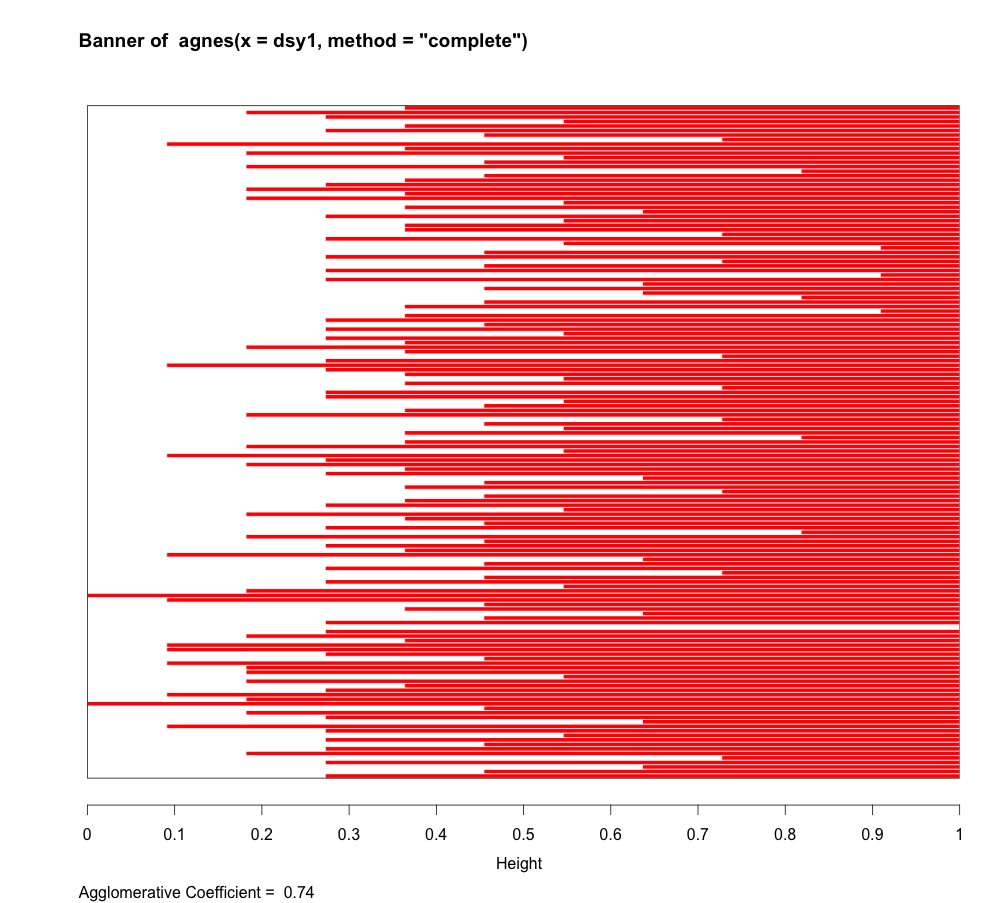
\includegraphics[scale = 0.35,angle = 0]{figures/banner.png}
  \caption[Sample Banner Agglomerative Clustering Results]{\normalsize{Sample Banner Agglomerative Clustering Results}}
  \label{fig:ban1}
  \end{figure}
  
  The white lines extending to the right represent clusters which differ
  from each other. After running the bottom up clustering method for a
  number of trials, the agglomerative coefficient was always between .73
  and .8, indicating that as the height for which the clusters should stop
  combining. Again, Figure 1 demonstrates that at that height, around 8
  clusters are have clearly seperated.
  
  \subsection*{OR}\label{or}
  \addcontentsline{toc}{subsection}{OR}
  
  Because urgent care centers have been significantly overlooked by
  sociologists studying medical practices, there was little theoretical
  guidance in selecting a likely number of subgroups for the cluster
  analysis, often the first step in such examinations. Similarly, because
  I am interested in understanding how an unsupervised analysis of patient
  data will reveal trends, rather than imposing them onto the data, it was
  particularly important to the investigation that the number of clusters
  be both mathematically achievable and substantively small enough for
  analysis while still remaining unsupervised. The general rule of thumb
  for cluster analysis suggested by Mardia, Kent and Bibbby (1997)
  stipulates that the number of clusters k is approximately the square
  root of n / 2. However, in the case of our comparably small sample of
  urgent care visitors recorded in the NAMCS data set, such a rule would
  indicate at least 30 clusters---clearly not a workable number to make
  sense of patterns in urgent care patients and their use.
  
  Instead, to estimate a k which would produce heterogeneous groups while
  still remaining theoretically enlightening, I began with non-guided
  hierarchal clustering of samples of 200 visits to urgent care centers
  randomly chosen from the data. Using the Gower methodology of finding
  the distance between dissimilar variable types, I calculated the
  distance matrix between the various observations for each sample. These
  distance measures were then used as the input to a hierarchal clustering
  algorithm which attempted to minimize the distance between observations
  within the same groups while maximizing the distance between them.
  Figure 1 shows the `banner' for the initial agglomerative cluster
  methods for the behavioral variables, and can be understood as a
  graphical representation of the points at which a cluster breaks away
  from the pack of observations. The white lines extending to the right
  represent clusters at their separation point, where larger red areas
  between white lines indicate stronger outside group variance.
  
  It should be noted that though the analyses were performed in two waves,
  the clusters should be examined with each other in mind, and I have
  included some of the key demographic variables in with the behavioral
  variables to that end. {[}OH YEAH, THIS IS GOING IN THE APPENDIX{]}
  
  \emph{Figure 2. Color coded clusters.}
  
  Figure 1 above shows the typical spread of the behavioral parameters'
  clusters, and is useful for keeping the proportions of clusters in mind.
  
  \backmatter
  
  \chapter{References}\label{references}
  
  \noindent
  
  \setlength{\parindent}{-0.20in} \setlength{\leftskip}{0.20in}
  \setlength{\parskip}{8pt}
  
  \hypertarget{refs}{}
  \hypertarget{ref-namcs}{}
  NAMCS/NHAMCS - Questionnaires, Datasets, and Related Documentation.
  (n.d.). Retrieved from
  \url{http://www.cdc.gov/nchs/ahcd/ahcd_questionnaires.htm\#documentation}
  
  \hypertarget{ref-CITE}{}
  Unknown. (). FIND cITATION. \emph{YOU DONT KNOW}.


  % Index?

\end{document}

